Im Folgenden sind die aufgenommenen Messwerte und die aus diesen
berechneten Größen vorwiegend tabellarisch aufgetragen. Die jeweiligen Fehler der berechneten Werte, wurden mit den angegebenen, in römischen Zahlen nummerierten Fehlergleichung nach Gauß bestimmt, welche sich in 
\cref{sec:Fehlerrechnung} befinden.
An entsprechender Stelle sind Erklärungen zu den Werten und Rechnungen gegeben.\\

In den Abschnitten \ref{sec:Auswertung_Wheatstone} bis \ref{sec:Auswertung_Induktivität_Maxwell} wird, wie in \cref{sec:Durchführung}
beschrieben ein Potentiometer verwendet, um den Widerstand $R_{3}$ einzustellen. Mit dem Maximalwiderstand \\$R_{max} = \SI{1003}{\ohm}$
des Potentiometers, erhält man den Widerstand $R_{4}$ als:
\begin{empheq}{equation}
	\label{eq:R4}
	R_{4} = R_{max} - R_{3} = \SI{1003}{\ohm} - R_{3}
\end{empheq}

\subsection{Bestimmung eines Widerstandes mit der Wheatstonebrücke}
\label{sec:Auswertung_Wheatstone}

	Bei dieser Messung wurde der unbekannte Widerstand \emph{Wert 10} vermessen.
	Der am Potentiometer eingestellte Widerstand $R_{3}$, der Quotient aus diesen und den nach \cref{eq:R4} berechneten
	Widerständen $R_{4}$, die jeweiligen
	Abgleichwiderstände $R_{2}$ und die mit Hilfe von \cref{eq:Rx} aus diesen
	berechneten Werte für $R_{x}$ sind in \cref{tab:Wheatstone} zu finden.
	
	\begin{table}[!h]
	\centering
	\begin{tabular}{|c|c|c|c|}
		\hline
		Widerstand & Widerstand   & Widerstand  & Widerstand  \\ 
		$R_{2}\,[\si{\ohm}]$ & $R_{3}\,[\si{\ohm}]$ & $\frac{R_{3}}{R_{4}}\,[\si{\ohm}]$ & $R_{x}\,[\si{\ohm}]$\\\hline\hline
		\num{332.000}  & \num{421.000}  & \num{0.723(4)}  & \num{240(1)} \\
		\num{664.000}  & \num{266.000}  & \num{0.361(2)}  & \num{240(1)} \\
		\num{1000.000}  & \num{195.000}  & \num{0.241(1)}  & \num{241(1)} \\
		\hline
	\end{tabular}
	\caption{Werte der Messung an der Wheatstonebrücke \label{tab:tab:Wheatstone}}
\end{table}

	Der Mittelwert der errechneten Werte für $R_{x}$ ergibt sich aus den Messwerten zu,
	\begin{empheq}{equation}
		\mean{R_{x}} = \SI{240.4(7)}{\ohm}
	\end{empheq}
	wobei der Fehler mit \cref{std:Mittel} bestimmt wurde.
	
\subsection{Bestimmung von Kapazitäten mit einer Kapazitätsmessbrücke}
\label{sec:Auswertung_Kapazitaet}
	In den zwei nachfolgenden Abschnitten werden die Kapazitäten einer 
	idealen und einer realen Kapazität mit Hilfe einer Kapazitätsmessbrücke
	bestimmt.
	
	\subsubsection{Bestimmung einer idealen Kapazität}
	\label{sec:Auswertung_Kapazität_ideal}
		Aus den in \cref{tab:Kapazitaet_ideal} gelisteten Messwerten für die Abgleichkapazitäten
		$C_{2}$, den am Potentiometer eingestellten Widerständen $R_{3}$ und den mit \cref{eq:R4} 
		aus diesen bestimmten $R_{4}$ wurden die ebenfalls in \cref*{tab:Kapazitaet_ideal} dargestellten
		unbekannten Kapazitäten $C_{x}$ (\emph{Wert 3}) unter Verwendung von \cref{eq:Kapazitaet_C} bestimmt. 
		
		\begin{table}[!h]
	\centering
	\begin{tabular}{|c|c|c|c|}
		\hline
		Kapazität & Widerstand & Quotient & Widerstand\\
		$C_{2}\,[\si{\nano\farad}]$ & $R_{3}\,[\si{\ohm}]$ & $\frac{R_{3}}{R_{4}}$ & $C_{x}\,[\si{\nano\farad}]\,\cref{std:Quotient}$\\\hline\hline
		\num{994(2)}  & \num{705}  & \num{2.37(1)}  & \num{420(2)} \\
		\num{750(2)}  & \num{640}  & \num{1.763(9)}  & \num{425(2)} \\
		\num{597(1)}  & \num{589}  & \num{1.423(7)}  & \num{420(2)} \\
		\hline
	\end{tabular}
	\caption{Werte der Messung einer idealen Kapazitätan der Kapazitätsmessbrücke \label{tab:Kapazitaet_ideal}}
\end{table}	
	
		Als Mittelwert der unbekannten Kapazität $C_{x}$ erhält man hieraus,
		\begin{empheq}{equation}
			\mean{C_{x}} = \SI{422(1)}{\nano\farad}
		\end{empheq} 
		mit dem Fehler nach \cref{std:Mittel}.
		
	\subsubsection{Bestimmung einer realen Kapazität}
	\label{sec:Auswertung_Kapazität_real}
		
		Für die Bestimmung einer realen Kapazität (\emph{Wert 9}) wird, anderes als bei der einer idealen Kapazität, ein
		Stellglied $R_{2} = \SI{500(15)}{\ohm}$ benötigt. Die anderen bekannten Größen sind analog zu
		 \cref{sec:Auswertung_Kapazität_ideal} zusammen mit den aus diesen 
		berechneten unbekannten Größen, die Kapazität $C_{x}$ bestimmt durch \cref{eq:Kapazitaet_C} und deren
		 Wirkwiderstand $R_{x}$ bestimmt durch \cref{eq:Rx} in 
		\cref{tab:Kapazitaet_real} eingetragen. 
	
		\begin{table}[!h]
	\centering
	\begin{tabular}{|c|c|c|c|c|}
		\hline
		Kapazität & Widerstand & Quotient & Kapazität & Widerstand\\
		$C_{2}\,[\si{\nano\farad}]$ & $R_{3}\,[\si{\ohm}]$ & $\frac{R_{3}}{R_{4}}$ & $C_{x}\,[\si{\nano\farad}]\,\cref{std:Quotient}$ & $R_{x}\,[\si{\ohm}]\,\cref{std:Quotient}$\\\hline\hline
		\num{994(2)}  & \num{632}  & \num{1.704(9)}  & \num{584(3)}  & \num{852(4)} \\
		\num{750(2)}  & \num{586}  & \num{1.405(7)}  & \num{534(3)}  & \num{703(4)} \\
		\num{597(1)}  & \num{561}  & \num{1.269(6)}  & \num{470(3)}  & \num{635(3)} \\
		\hline
	\end{tabular}
	\caption{Werte der Messung einer idealen Kapazitätan der Kapazitätsmessbrücke \label{tab:Kapazitaet_real}}
\end{table}

		Die Mittelwerte der unbekannten Größen $C_{x}$ und $R_{x}$ ergeben sich somit zu:
		\begin{empheq}{equation}
				\mean{C_{x}} = \SI{529(2)}{\nano\farad} \quad\ \text{und}\ \quad \mean{R_{x}} = \SI{730(2)}{\ohm}
		\end{empheq}  
		Der Fehler wurde jeweils mit Hilfe von \cref{std:Mittel} bestimmt.
\subsection{Bestimmung von Induktivitäten}
\label{sec:Auswertung_Induktivität}

	Nachfolgend wird eine reale Induktivität (\emph{Wert 16}) zunächst mit Hilfe einer Induktivitätsmessbrücke
	und anschließend mit einer Maxwellbrücke vermessen. Bei beiden Untersuchungen wird 
	ein Stellglied $R_{2} = \SI{1000}{\ohm}$ verwendet.
	
	\subsubsection{Bestimmung Mittels einer Induktivitätsmessbrücke}
	\label{sec:Auswertung_Induktivität_Messbrücke}
	
		Die verwendeten Abgleichinduktivitäten $L_{2}$, der am Potentiometer eingestellten Widerstand
		$R_{3}$ sowie die Quotienten aus diesen und den nach \cref{eq:R4} berechneten Widerständen $R4$
		und die mit Hilfe von \cref{eq:Induktivitaet_L} und \cref{eq:Rx} berechneten unbekannten $L_{x}$
		 und $R_{x}$ sind in \cref{tab:Induktivitaet_Bruecke} zu finden.    
		
		\begin{table}[!h]
	\centering
	\begin{tabular}{|c|c|c|c|c|}
		\hline
		Induktivität & Widerstand & Widerstand & Induktivität& Widerstand\\
		$L_{2}\,[\si{\milli\henry}]$ & $R_{3}\,[\si{\ohm}]$ & $\frac{R_{3}}{R_{4}}$ & $L_{x}\,[\si{\milli\henry}]$ & $R_{x}\,[\si{\ohm}]$\\\hline\hline
		\num{20.1}  & \num{305}  & \num{0.437(2)}  & \num{8.78(4)}  & \num{436(13)} \\
		\num{27.5}  & \num{321}  & \num{0.471(2)}  & \num{12.94(6)}  & \num{471(14)} \\
		\hline
	\end{tabular}
	\caption{Werte der Messung einer realen Induktivität mit einer Induktivitätsmessbrücke \label{tab:Induktivitaet_Bruecke}}
\end{table}
		
		Die aus diesen Werten bestimmten Mittelwerte der Unbekannten Größen, mit den Fehlern nach \cref{std:Mittel} sind:
		\begin{empheq}{equation}
				\label{eq:LxRx_Brücke}
				\mean{L_{x}} = \SI{10.86(4)}{\milli\henry} \quad\ \text{und}\ \quad \mean{R_{x}} = \SI{454(10)}{\ohm}
		\end{empheq}		
		
		
	\subsubsection{Bestimmung Mittels einer Maxwellbrücke}
	\label{sec:Auswertung_Induktivität_Maxwell}
		
		Bei der Bestimmung der Induktivität $L_{x}$ und deren Wirkwiderstand $R_{x}$ werden 
		nur der am Potentiometer eingestellte Widerstand $R_{3}= \SI{210(6)}{\ohm} $, der mit \cref{eq:R4} 
		daraus bestimmte Widerstand $R_{4} = \SI{793(30)}{\ohm}$ und die verwendete Kapazität $C_{4} = 
		\SI{994}{\nano\farad}$  benötigt. Mit \cref{eq:Induktivitaet_Maxwell_L} und \cref{eq:Rx}
		sowie dem Stellglied $R_{2}$ erhält man:
		\begin{empheq}{equation}
				\label{eq:LxRx_Maxwell}
				{L_{x}} = \SI{0.209(9)}{\henry} \quad\ \text{und}\ \quad {R_{x}} = \SI{265(15)}{\ohm}
		\end{empheq}
		Die Fehler dieser beiden Größen wurden dabei mit \cref{std:Maxwell_L}
		beziehungsweise \cref{std:Maxwell_R} bestimmt.
		
\subsection{Bestimmung der Frequenzabhängigkeit der Brückenspannung}
\label{sec:Auswertung_Frequenz}
	
	Für die Durchführung dieses Versuches wurde eine Wien-Robinson-Brücke, mit folgenden Bauteilen
	verwendet:
	\begin{empheq}{align*}
			R'&= \SI{500}{\ohm}\\
			R &= \SI{332}{\ohm} \\
			C &= \mean{C_{x}} \footnotemark = \SI{242(1)}{\nano\farad}
	\end{empheq}		
\footnotetext{Aus \cref{sec:Auswertung_Kapazität_ideal}}		
	
	Die eingestellten Generatorfrequenzen $\nu$ sind zusammen mit den jeweils gemessenen, doppelten Amplituden der, 
	Brückenspannungen $U_{Br}$ in \cref{tab:Frequenz} zu finden. Die doppelte Amplitude der Generatorspannung wurde zu
	$_{S} = \SI{4.250(1)}{\volt}$ gemessen. 
	
	\begin{table}[!h]
	\centering
	\begin{tabular}{|c|c||c|c|}
		\hline
		Frequenz & Brückenspannung & Frequenz & Brückenspannung\\
		$\nu\,[\si{\hertz}]$ & $U_{Br}\,[\si{\volt}]$ & $\nu\,[\si{\hertz}]$ & $U_{Br}\,[\si{\volt}]$\\\hline\hline
		\num{20.3(1)}  & \num{1.438(1)} &\num{6010.3(1)}  & \num{1.025(1)} \\
		\num{350.4(1)}  & \num{0.944(1)} &\num{7000.3(1)}  & \num{1.050(1)} \\
		\num{670.3(1)}  & \num{0.469(1)} &	\num{8000.3(1)}  & \num{1.075(1)} \\
		\num{800.3(1)}  & \num{0.319(1)} &	\num{10030.3(1)}  & \num{1.094(1)} \\
		\num{900.3(1)}  & \num{0.209(1)} &	\num{15000.0(1)}  & \num{1.100(1)} \\
		\num{1000.3(1)}  & \num{0.119(1)} &\num{20030.3(1)}  & \num{1.075(1)} \\
		\bfseries\num[detect-weight]{1110.3(1)}  & \bfseries\num[detect-weight]{0.033(1)} &	\num{23100.0(1)}  & \num{1.044(1)} \\
		\num{1400.3(1)}  & \num{0.178(1)} &\num{25000.0(1)}  & \num{1.038(1)} \\
		\num{2000.3(1)}  & \num{0.463(1)} &	\num{27000.0(1)}  & \num{1.019(1)} \\
		\num{3200.3(1)}  & \num{0.772(1)} &\num{28000.0(1)}  & \num{1.013(1)} \\
		\num{4000.3(1)}  & \num{0.888(1)} &\num{29000.0(1)}  & \num{1.006(1)} \\
		\num{5000.3(1)}  & \num{0.975(1)} &\num{30100.0(1)}  & \num{0.994(1)} \\
		\hline
	\end{tabular}
	\caption{Generatorfrequenzen und gemessene Brückenspannungen \label{tab:Frequenz}}
\end{table}
	
	Dabei sind die hervorgehobenen Werte die Frequenz $\nu_{0} = \SI{1110.3(1)}{\hertz}$ bei der die minimale Spannung
	$U_{0} = \SI{0.033(1)}{\volt}$ gemessen wurde. Die durch Division von \cref{eq:Frequenz_0} durch $2\pi$ theoretisch 
	bestimmte Frequenz, bei der die 
	Brückenspannung verschwindet beziehungsweise minimal wird ist $\nu_{0,theo} = \SI{1137(3)}{\hertz}$ mit dem Fehler nach \cref{std:Frequenz_0}.\\     
	
	In \cref{fig:WienRobinson} ist der Quotient $\frac{U_{Br}}{U_{S}}$ gegen 
	den Quotienten  $\Omega = \frac{\nu}{\nu_{0}}$ halblogarithmisch aufgetragen, wobei die Zähler dieser Quotienten,
	jeweils die Werte aus \cref{tab:Frequenz} darstellen. Des Weiteren ist noch die Theoriekurve dieses Verlaufes, bestimmt durch radizieren von \cref{eq:UBr_US}, eingezeichnet.  
		
	\begin{figure}[!h]
		\centering
		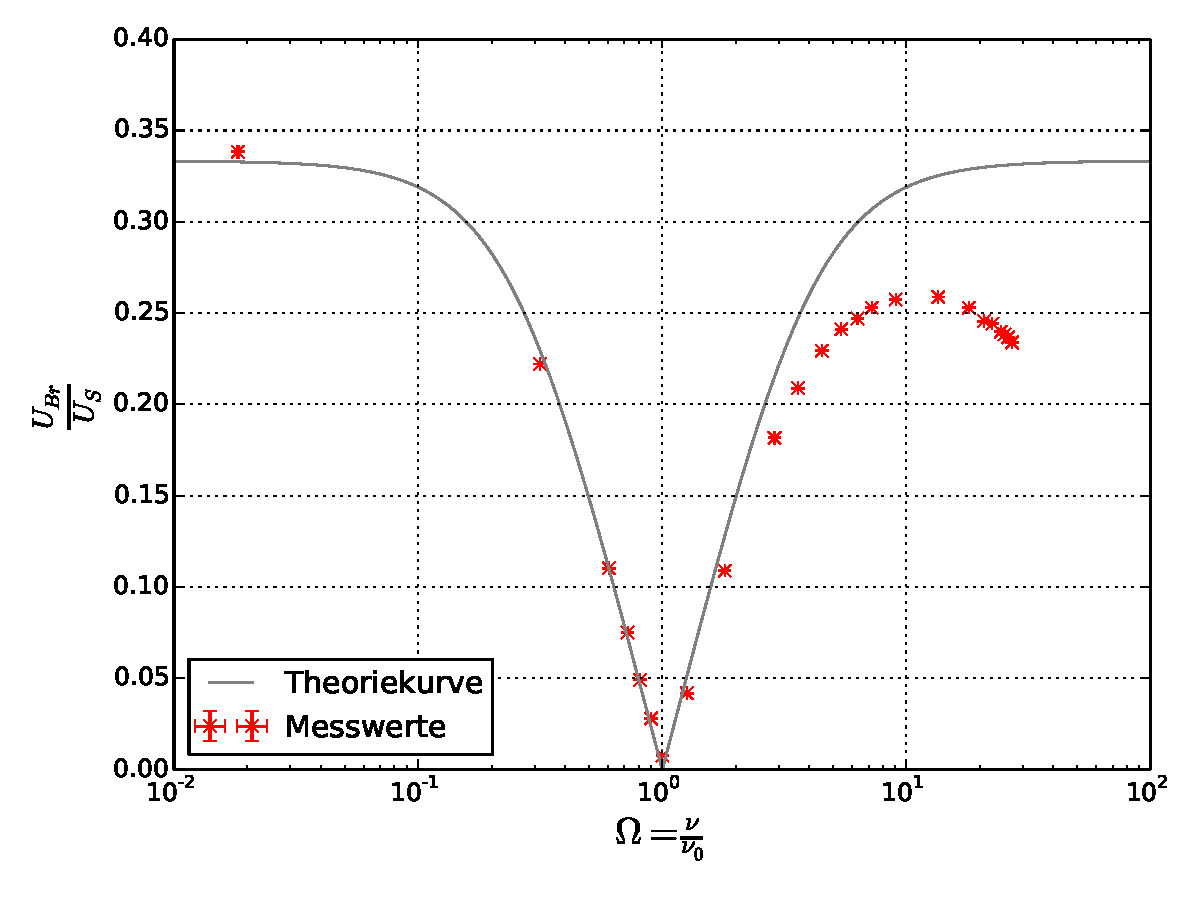
\includegraphics[scale=0.75]{Grafiken/WienRobinson.pdf}
		\caption{Messwerte und Theoriekurve der Spannungs- und Frequenzverhältnisse}
		\label{fig:WienRobinson}
	\end{figure}

\subsubsection{Bestimmung des Klirrfaktors eins Frequenzgenerators}
\label{sec:Auswertung_Klirrfaktor} 
	
	Den Klirrfaktor eines Frequenzgenetrators erhält, unter der Annahme $\displaystyle U_{2}^{2} = \sum_{i=2}^{n} U_{i}^{2}$,
	nach \cref{eq:Klirrfaktor}, durch die Gleichung:
	\begin{empheq}{equation}
		k = \dfrac{U_{2}}{U_{1}}
		\label{eq:Klirrfaktor2}
	\end{empheq}     
	
	Wobei sich die doppelte Amplitude der ersten Oberschwingung $U_{2}$ durch \cref{eq:U2} ergibt.
    Damit ist die doppelte Amplitude der ersten Oberwelle $U_{2} = \SI{0.221(7)}{\volt}$ mit dem Fehler nach \cref{std:Oberwelle},
	woraus sich der Klirrfaktor
	\begin{empheq}{equation}
		\label{eq:Klirrfaktor_Wert}
		k = \num{0.052(2)}
	\end{empheq}	
	ergibt, dessen Fehler unter Verwendung von \cref{std:Klirrfaktor} berechnet wurde.